\documentclass[12pt, a4paper]{scrartcl}

%=======================
%       IMPORTS
%=======================
\usepackage{a4wide}
\usepackage{fontspec}
\usepackage{unicode-math}
\usepackage{microtype}
\usepackage{polyglossia}
\usepackage{csquotes}

\usepackage[
    backend = biber,
    style = ieee-alphabetic
]{biblatex}

\usepackage[dvipsnames]{xcolor}
\usepackage{graphicx}

\usepackage{caption}
\usepackage{subcaption}
\usepackage{tocloft}

\usepackage{acronym}

\usepackage{booktabs}
\usepackage{enumitem}

\usepackage{tikz}
\usepackage{pgf-pie}

\usepackage[
    breaklinks = true,
    hidelinks,
    unicode = true,
    pdfencoding = auto
]{hyperref}

%=======================
%     PACKAGE SETUPS
%=======================
% Language Setup
\setdefaultlanguage{english}

% Font Setup
\setmainfont{TeX Gyre Pagella}
\setmathfont{TeX Gyre Pagella Math}

% Pfad für Grafiken
\graphicspath{graphics/}

% Styleregeln
\widowpenalty10000  % Vermeidet einzelne Zeilen eines Absatzes zu Beginn einer Seite
\clubpenalty10000   % Vermeidet einzelne Zeilen eines Absatzes am Ende einer Seite
\addtocontents{toc}{\protect\sloppy}
\setcounter{tocdepth}{3}

% Hyperref
\hypersetup{
    colorlinks,
    linkcolor={black},
    citecolor={blue!50!black},
    urlcolor={blue!80!black},
    pdftitle={Server Consolidation Techniques in Virtualized Data Centers},
    pdfauthor={Leon Richardt}
}

% BibLaTeX
\addbibresource{{../green.bib}}

%=======================
%    DOCUMENT START
%=======================
\begin{document}

% Deaktiviere Seitenzahlen	
\pagenumbering{gobble}

% Titelseite
\begin{titlepage}
    \centering
    \thispagestyle{empty}

    \begin{center}
        \includegraphics[width=0.9\textwidth]{uos.pdf}
    \end{center}

    \LARGE{\textsc{Institut für Informatik\\Arbeitsgruppe Verteilte Systeme}}
    \vfill
    \LARGE{\textit{Seminar Green Networking}}\\
    \vspace{8mm}
    \huge{\textbf{Server Consolidation Techniques in Virtualized Data Centers}}\\
    \vspace{9mm}
    \LARGE{Leon Richardt}\\
    \vspace{0.2cm}
    % TODO: Matrikelnummer
    \normalsize{Matrikelnummer}\\
    \vspace{4cm}
    \large{Wintersemester 2019/2020}\\
    \vspace{0.2cm}
    \large{19. Dezember 2019}
    \vfill
\end{titlepage}
\newpage

% Inhaltsverzeichnis
\tableofcontents
\newpage

\pagestyle{plain}
\pagenumbering{arabic}  % Starte Seitennummerierung

\section{Introduction}\label{sec:intro}
In recent years, companies such as Google \cite{google_cloud_2019}, Amazon \cite{amazon_ec2_2019}, and Microsoft \cite{microsoft_azure_2019} have continually expanded their cloud computing platforms in order to keep up with an increasing demand for faster and more reliable online services.
They advertise scalability and stability for services running on their platforms.
Since energy usage by data centers kept rising during the early 2000s \cite[25-32]{brown_report_2008} (roughly doubling over the course of five years), cloud computing providers were incentivized to develop solutions that keep costs low but reliability and performance high.
These two goals seem contradictory at first: An obvious way to achieve reliability is the introduction of redundancy which in turn leads to an increase in power consumption.
Indeed, studies have found that average server CPU utilization is between 10\% and 50\% for about 80\% of the time \cite{barroso_epc_2007}.
Server virtualization and consolidation techniques provide possibilities to address these issues and find a solution that is energy-efficient as well as financially feasible \cite{varasteh_survey_2017}.

In this paper, we give an overview on how these methods can be applied to large-scale systems.
To start off, Section~\ref{sec:principles} gives a brief introduction to the basic model underlying virtualized data centers.
Section~\ref{sec:optimization} presents a number of different system parameters consolidation strategies could optimize for.
Finally, Section~\ref{sec:conclusion} summarizes the obtained results and gives an outlook on possible future developments.

\section{Principles}\label{sec:principles}
In this section, we lay out some of the fundamentals required to understand the idea of saving power through server virtualization.
Furthermore, we introduce the notion of \acp{VM} and how they can be used to efficiently run a large number of workloads on a smaller number of \acp{PM}.

A key idea for saving power through server consolidation lies in reducing the number of idle machines in the data center.
A naive approach might consider running all tasks on a single system.
However, this is not a viable practice in every scenario; often due to security sensitive applications which require stronger isolation.
\acp{VM} provide a possible solution to this problem.

\subsection{Power Consumption in Data Centers}\label{sec:power-con}
According to \cite{iea_analysis_2019}, the global power consumption in data centers amounted to 198~TWh in 2018 which is about 1\% of total global electricity demand.
Although data center workloads are expected to triple by 2021, power consumption is projected to stay constant over the same period of time.
This development can be attributed to advances in software and hardware components.
One software solution, virtualization, will be further discussed in this paper.

In data centers, server hardware is not the only factor requiring power.
For example, a significant percentage of power usage is accounted for by the cooling system.
\autoref{fig:power-dist} presents a breakdown of the most relevant elements.

\begin{figure}
    \centering
    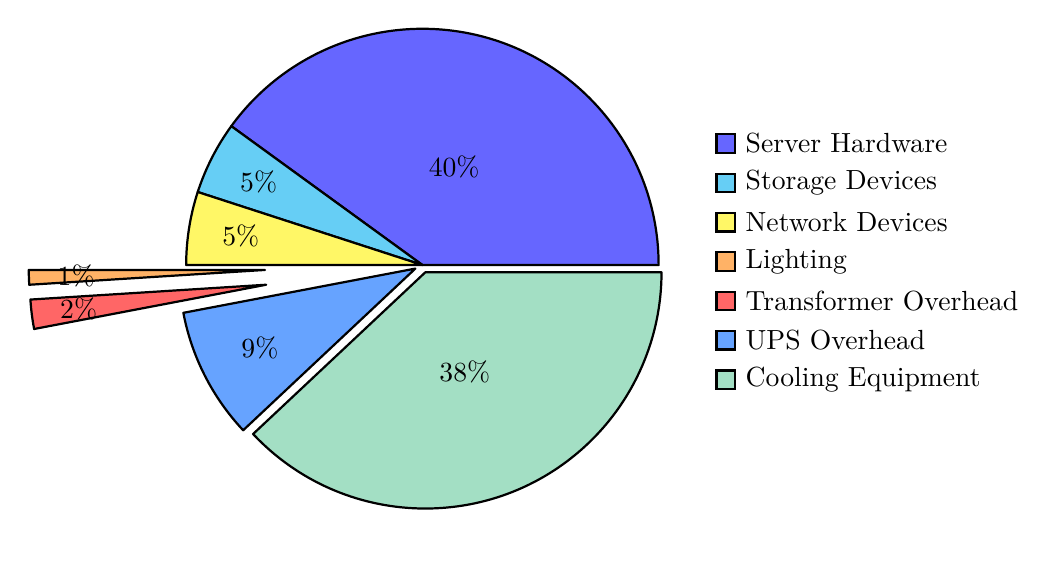
\begin{tikzpicture}
        \pie[
                radius = 3,
                text = legend,
                explode = {0, 0, 0, 2, 2, 0.1, 0.1}
            ]
            {
                40/{Server Hardware},
                5/{Storage Devices},
                5/{Network Devices},
                1/{Lighting},
                2/{Transformer Overhead},
                9/{UPS Overhead},
                38/{Cooling Equipment}
            }
    \end{tikzpicture}

    \caption{Average distribution of power consumption by different data center components, see \cite{masanet_estimating_2011}.}
    \label{fig:power-dist}
\end{figure}

\begin{description}
    \item[Server Hardware]
        Closely attached (\enquote{internal}) server components, such as the CPU and memory.

    \item[Storage Devices]
        External storage devices, generally consisting of \acp{HDD} and \acp{SSD}.

    \item[Network Devices]
        Devices supporting the local network layout, like routers or switches.

    \item[Lighting]
        Although a comparably small point, lighting equipment in data centers must also be considered.

    \item[Transformer Overhead]
        To generate the required alternating voltages, transformers may need to be used.
        In doing so, however, power loss will occur.
        \textcite{masanet_estimating_2011} assume an efficiency rate of 95\%.

    \item[UPS Overhead]
        Uninterruptible power supplies\acused{UPS} (\acp{UPS}) are designed to protect the data center equipment from sudden power outages.
        They provide power from battery until the main circuit, or a backup system, can be restored.
        In \cite{masanet_estimating_2011}, this redundancy is assumed to incur a power loss of about 20\%.

    \item[Cooling Equipment]
        The largest auxiliary consumer of energy is the cooling infrastructure.
        It includes equipment such as air conditioners, coolant pumps, fans, and water chillers.
\end{description}

Power consumption can therefore be modelled as a function of the energy usage of server hardware, storage devices, network devices, and infrastructure equipment.

\subsection{Virtual Machines}
\textcite{popek_vm_1974} define a \ac{VM} to be \enquote{an efficient, isolated duplicate of the real machine}.
In practice, this property concerns the ability to execute any program that can also be executed by a suitable unvirtualized machine.
\acp{VM} are created and managed by a \ac{VMM}: a piece of software that is responsible for distributing the available physical resources (e.g.\ CPU time, memory, or network bandwidth) to the hosted \acp{VM}.
Some authors also use the term \emph{hypervisor} instead of \ac{VMM}.

A distinction must be made between Type-1 (\emph{native, classic system}) and Type-2 (\emph{hosted}) \acp{VMM}.
While Type-1 \acp{VMM} run directly on the host's hardware, Type-2 \acp{VMM} run on top of the host operating system.
It follows that Type-1 \acp{VMM} must implement their own hardware-specific drivers whereas Type-2 \acp{VMM} can rely on the host operating system to provide such functionality.
An example for a native \ac{VMM} is Xen \cite{xen}; an example for a hosted \ac{VMM} is VirtualBox \cite{virtualbox}.
Some software, such as KVM \cite{kvm}, cannot easily be classified into one of these two categories.

\subsubsection{VM Migration}\label{sec:migration}
A key feature of \acp{VM} is the possibility to migrate an existing \ac{VM} to another physical machine.
In order to perform a successful migration, different aspects of the \ac{VM} image need to be considered:
\begin{enumerate}
    \item
        The \emph{internal state}.
        This includes the current state of the virtual CPU and memory as well as networking and storage adapters.
        
    \item
        The \emph{external state}.
        This item concerns the \ac{VM}'s use of external devices, such as USB devices, removable media or networking equipment.
\end{enumerate}
One possible procedure to migrate a \acp{VM} is described by \textcite{clark_migration_2005}.
It is designed to incur minimal overhead on the overall system performance:
\begin{enumerate}
    \item
        Select a source \ac{VM} and a destination \ac{PM} (\emph{target}) to migrate to.
        (Potentially aided by certain optimization criteria, described in section \ref{sec:optimization}.)

    \item
        Iteratively copy memory to the target.
        Since transferring the memory state usually has the biggest impact on performance, this is done while the \ac{VM} is still running.
        Memory pages that are modified after they have been copied are marked to be sent again.

    \item
        Stop the \ac{VM} and transfer all non-memory state.
        Send any pages that are still marked for retransmission.

    \item
        Resume the \ac{VM} image on the target.
\end{enumerate}
The technique used in Step 2 is known as \emph{iterative pre-copying}.
At the beginning of the migration process, many pages need to be copied to the target.
Memory pages that have been modified during an iteration are sent to the target again.
Assuming typical workloads, increasingly less pages will have been modified in each iteration (since each iteration completes quicker than the previous one).
This also means that the amount of differing memory pages between source and destination is reduced in each iteration.
Pre-copying is stopped once a sufficiently low threshold of deviation has been achieved.
Alternatively, the process may also be stopped when no significant reduction in the number of pages to transfer can be achieved.

By migrating \acp{VM} from a large number of moderately busy \acp{PM} to a smaller number of heavily loaded \acp{PM}, idle machines can be put into low-power modes or shut down entirely.
This can provide significant power savings.

\section{Optimization Parameters}\label{sec:optimization}
As mentioned above, \ac{VM} migration provides an useful mechanism to balance workloads across multiple \acp{PM}.
One can imagine numerous ways to measure workloads:
CPU utilization, IO utilization, or service reliability could come to mind.
This section presents a number of parameters to consider when selecting source \acp{VM} and target \acp{PM} for migration.

\subsection{Hardware Utilization}
In \cite{gmach_resource_2009}, \citeauthor{gmach_resource_2009} introduce a load balancing model and policies that optimize CPU and memory utilization in server pools.
A \ac{PM} is defined to be overloaded if CPU or memory load exceed a previously specified maximum threshold.
In contrast, the \emph{system} is said to be underloaded if the average CPU and memory usage stay below a certain minimum threshold.

The authors describe a number of rebalancing policies a migration manager can employ:
\begin{description}
    \item[Reactive]
        A reactive policy responds when a violation of either threshold is detected.

        When an overload situation occurs, the migration manager determines a migration candidate on the overloaded server.
        That \ac{VM} is then transferred to the least loaded server with adequate resources for the workload.
        If no suitable \ac{PM} for the workload exists at the time of migration, a new server is started.

        In an underload scenario, the migration manager determines the least loaded \ac{PM} and tries to transfer all running \acp{VM} in such a way that no server will be overloaded after the migration.

    \item[Trace-Based]
        With this policy, the migration manager will periodically use historical data to predict the expected workload for the next interval.
        At the start of every interval, traces of past workloads are considered to construct a workload distribution fitting the historical data.
        Current system load is not taken into account.  
        In \cite{gmach_resource_2009}, the authors decided to select a 4~h rebalancing interval for their case study.

    \item[Reactive/Trace-Based]
        This policy combines the previous strategies:
        Traces are used to rebalance the workload at the start of every interval.
        In the case of a threshold violation, the migration manager is invoked to resolve the situation as described in the Reactive policy.

    \item[Reactive/On-Demand Balancing]
        This policy works like the previous approach.
        However, the trace-based rebalancing is \emph{not only} applied periodically but also whenever servers are being under-utilized.
\end{description}

The authors measure the effectiveness of these policies by counting the CPU/memory threshold violations per hour.
Clearly, the \enquote{success} of these policies is dependent on the threshold values selected by the data center operators.
When operating on strict thresholds (high underload and low overload limits), the pure Reactive and pure Trace-Based policies produce the most violations.
Especially the Trace-Based migration policy is prone to violations since deviations from the traces will not lead to a change in allocation behavior.
Therefore, employing a purely Trace-Based policy only makes sense when the workload adheres to strict periodic patterns.

The combined approaches seem to be much more robust:
They can leverage historical information to overprovision \acp{PM} for the next interval.
In case the trace data still turns out not to be applicable to the current workload scenario, the migration manager may resolve violations by performing further migrations.

\subsection{Network Traffic}
\textcite{meng_traffic_aware_2010} assert that modern data center applications are increasingly communication-intensive whereas existing \ac{VM} placement strategies solely base their decisions on factors such as CPU and memory utilization.

In order to study the problem, they assume the existence of \(n\) \acp{VM} and \(n\) slots (one slot represents the ability to place a \ac{VM} on a \ac{PM}).
They further assume that the number of slots any given server can host has been decided by \enquote{traditional} planning tools, i.e.\ tools that only consider CPU/memory utilization.
Let \(D_{ij}\) be the traffic rate between two \acp{VM} \(v_i\) and \(v_j\), and \(C_{ij}\) the communication cost between the slots \(s_i\) and \(s_j\).
\footnote{In \cite{meng_traffic_aware_2010}, the number of switches between two slots is chosen as a metric for the communication cost.}
Additionally, an external traffic rate \(e_i\) is defined for every \ac{VM}, as well as an external communication cost \(g_i\) between slot \(s_i\) and the network gateway.

The problem is then to find a bijective VM-to-slot mapping \(\pi \colon [1, \dots, n] \to [1, \dots, n]\) such that the expression
\[
    \underbrace{\sum_{i, j = 1, \dots, n} D_{ij} C_{\pi(i) \pi(j)}}_\text{Total internal cost}
    + \underbrace{\sum_{i = 1}^{n} e_i g_{\pi(i)}}_\text{Total external cost}
\]
is minimal.
The authors prove that finding an optimal mapping is NP-hard but also propose the approximation algorithm \emph{Cluster-and-Cut} with time complexity \(O(n^4)\).

The general idea of the algorithm is described as follows:
Based on their mutual communication rate, \acp{VM} are classified into clusters with regard to their traffic rate.
Likewise, slots with low intercommunication cost are clustered with the same size.
Each \ac{VM} cluster is then recursively mapped to a slot cluster.
The algorithm aims to place \ac{VM} pairs with high traffic between them onto slot pairs with low connection costs.

The authors find that the effectiveness of the algorithm is dependent on the network topology used in the data center.
They claim that topologies implementing load balancing, such as VL2 \cite{greenberg_vl2_2011}, do not profit as much as topologies that are load-ignorant.
According to an experimental case study conducted in \cite{meng_traffic_aware_2010}, the placement results of Cluster-and-Cut roughly lead to a 10\% improvement over two reference strategies, while also running faster.
This could be a major advantage when short migration intervals are desired.

\subsection{Thermal Efficiency}
As described in Section \ref{sec:power-con}, cooling systems are major power consumers in modern data centers.
Hence, some placement strategies are concerned with minimizing the required cooling effort (and thus, power consumption).
A naive approach might decide to place newly created \acp{VM} on those servers currently observing the minimal temperature.
However, \textcite{tang_thermal_aware_2007} argue that this course of action is not ideal.
Instead, they propose to minimize the total \emph{heat recirculation} inside the system.
Heat recirculation occurs when exhausted (hot) air from a server's ventilation outlet mixes with the newly supplied cold air from the ventilation system.
As a result, hotter air than originally supplied may enter the server inlets.
Since the temperature of this mixture is hard to predict, the ventilation system needs to cool down the supplied air further in order to provide a \enquote{buffer} for local hotspots.

In \cite{tang_thermal_aware_2007}, the authors show that minimizing heat recirculation is equivalent to minimizing the maximum inlet temperature of all servers.
In particular, this relationship is modelled by the expression
\[
    T_\text{in}
    = T_\text{sup}
    + \underbrace{D (a, a, \dots, a)^\intercal}_\text{Idle temperature}
    + \underbrace{b \cdot D \left( c_1, c_2, \dots, c_n \right)^\intercal}_\text{Workload temperature}
,\] 
where
\begin{itemize}[itemsep=0pt]
    \item 
        \(T_\text{in} = \left( t_{\text{in}_1}, \dots, t_{\text{in}_n} \right)\) is the vector of inlet air temperatures for each server,

    \item
        \(T_\text{sup} = \left( t_{\text{sup}_1}, \dots, t_{\text{sup}_n} \right)\) is the vector of air temperatures supplied by the ventilation for each server,

    \item
        \(D\) is a matrix describing the data-center-specific temperature circumstances,

    \item
        \(\left( c_1, \dots, c_n \right)\) is the vector describing the load of each server \(i\),

    \item
        and \(b\) is the \enquote{energy consumption per load} of a server (assumed to be constant for all servers).
\end{itemize}
Therefore, the aim is to find a load distribution \(\left( c_1, \dots, c_n \right)\) such that
\[
    \min\limits_{\left( c_1, \dots, c_n \right)}
    \left\{ \max\limits_{i = 1, \dots, n} \left\{ t_{\text{in}_i} \right\} \right\}
\] 
(the minimal peak temperature occurring in any load distribution) is reached.

They describe a genetic algorithm that approximates an optimal load distribution.
As a fitness function, the peak inlet temperature of all \acp{VM} is used.
Mutation is done by rebalancing the load distribution of a solution; crossover is done by exchanging a subset of \ac{VM} assignments.
Based on simulations conducted with this algorithm, the authors find a 20\% to 30\% reduction of energy cost compared to other algorithms at moderate load profiles.

\subsection{Evaluation}
The above results seem reasonably promising for data center operators.
However, there are some problems and open questions that still need to be answered.

\begin{description}
    \item[Applicability]
        It might not be trivial to decide whether a given optimization criterion is applicable to the expected workload of a data center.
        The Cluster-and-Cut algorithm, for example, can only be sensibly used when \acp{VM} in the same data center communicate with each other.
        While this may often be the case with high-performance computing applications, cloud computing providers like Google and Amazon will likely not profit from the metric.

    \item[Experimental Data]
        A common flaw in the studies and papers presenting new load balancing algorithms is the setting in which they were tested.
        Most of the time, simulations were run against traces of past workloads.
        Thus, the behavior of the policies in real-world data centers cannot truly be evaluated.

        This is understandable from a business standpoint:
        Putting production-critical applications at the risk of being compromised by untested load balancing algorithms is a tough sell.
        Minutes of downtime or service degradation can already lead to considerable financial damage.

    \item[Balancing Parameters]
        Different optimization parameters may be contradictory.
        For example, a hardware utilization-based and a network traffic-based algorithm can produce completely incoherent \ac{VM} placements.
        There is no \enquote{one-fits-all} model that could be applied to arbitrary workload profiles.
        Especially large data centers have lots of local parameters and conditions to consider.
        Development of a unified model is still an open problem; if it can be done at all \cite{meng_traffic_aware_2010}.

        Moreover, data center operators must balance the energy saving potential with existing \acp{SLA} among their customers.
        This aspect is examined more closely in \cite{gmach_resource_2009}.
\end{description}

\section{Conclusion \& Outlook}\label{sec:conclusion}
In this paper, we gave an overview of the power requirements in contemporary data centers and introduced the notion of a virtual machine.
We found that many factors contribute to high energy consumption.
In response to these observations, load balancing strategies concerning different optimization parameters were evaluated.
We assess that \ac{VM} migration is a useful tool to effectively distribute tasks among a number of servers.
In any case, quality of service must be maintained during \ac{VM} consolidation.

However, attention must be paid to the specific conditions present at a data center.
As demonstrated in Section \ref{sec:optimization}, many of the introduced balancing techniques heavily rely on special characteristics featured in a data center, e.g.\ the network topology, or the workloads running on the servers.
Nevertheless, some strategies may be applied more broadly.
For example, cooling considerations are likely relevant in almost every data center.

Comparing the performance of different migration strategies against each other is difficult since authors benchmark their implementations on different workloads and different hardware.
Hence, judging the presented techniques solely by the results attained in their original papers will likely not produce a representative ranking.  
An open problem is the development of a joint system model considering many optimization parameters in parallel.

A recent development regarding scalable data center operation are containerized applications, managed by tools like Kubernetes.
These systems also allow for task isolation and load scaling, while incurring less of an overhead than \acp{VM}.

Since cloud computing is projected to continue growing over the near future \cite{iea_analysis_2019}, one can expect load balancing and task placement technologies to stay relevant and be improved on over the next few years.

%Anhang

\clearpage
\section*{Appendix}
\addcontentsline{toc}{section}{Appendix}
\subsection*{List of Abbreviations}
\addcontentsline{toc}{subsection}{List of Abbreviations}
\begin{acronym}[LONG]
\acro{HDD}{hard disk drive}
\acro{SLA}{service-level agreement}
\acro{SSD}{solid-state drive}
\acro{UPS}{uninterruptible power supply}
\acro{VM}{virtual machine}
\acro{VMM}{virtual machine monitor}
\acrodefplural{UPS}[UPS]{uninterruptible power supplies}
\acro{PM}{physical machine}
\end{acronym}

% Bibliographie
\addcontentsline{toc}{section}{References}
\printbibliography

\end{document}
